%\section{Character of Energy and Electron Transfer Illustrated Using Pairs and Triples of Atoms}
\section{Geometric Influence on ICD and ETMD3  Illustrated Using Pairs and Triples of Atoms}
Approximating every system into pairs and triples of atoms is a very useful
first order approximation to both the investigation of energies and
decay widths of a larger system. Pairs and triples are combinations of
two and three atoms, respectively.
These atoms do not necessarily need to form bonds between each other or
even being close, but they are characterized according to fixed internal
coordinates. Each pair and triple can be described by its properties and
is in first order of approximation independent on further, eventually
present, atoms.

In case of the electronic decay processes one is interested in the
energies of the initial $E_{in}$ and the final states $E_{fin}$ of
the corresponding processes. They can be approximated to be

\begin{align}
 E_{in}  &= SIP(X{in}^\beta) \label{equation:E_in}\\
 E_{fin} &= SIP(X_{fin1}^\beta) + SIP(X_{fin2}^\beta) + \frac 1d
           \label{equation:E_fin}\\
 E_{sec} &= E_{in} - E_{fin} \label{equation:E_sec}
\end{align}
where $X_{in}$ denotes the initially ionized atom and
$X_{fin1}$ and $X_{fin2}$ describe the two ionized
atoms in the final state. $/beta$ denotes the decay channel characterized
by the total angular momenta of the ionized atoms in the pairs
and triples and $d$ denotes the interatomic distance between the atoms
$X_{fin1}$ and $X_{fin2}$. The initially ionized atom $X_{in}$ can
coincide with one or both of
the final state atoms
$X_{fin1}$ and $X_{fin2}$. As explained in
section \ref{xyz}, the distribution of the vacancies over the different
atoms determine the kind of electronic decay process. Hence, in an
Auger process all three atoms would coincide, for an ICD $X_{in}$
would coincide with one of $X_{fin1}$ and $X_{fin2}$ and for an \ac{ETMD}3
all ionized states are located on different atoms.

In all considered autoionization processes a second electron
is emitted with the kinetic energy $E_{sec}$. If $E_{sec}<0$, then
the final state energy is higher than the initial state energy and the
process is energetically not accessible.

The decay widths of the pairs and triples can be estimated with
different accuracy, but in general, the total decay width $\Gamma$ of
a system is the sum over the decay widths of all channels $\beta$ for
all possible pairs or triples $i$.

\begin{equation}
  \Gamma = \sum\limits_{i,\beta}\Gamma_{i,\beta}
\end{equation}


\subsection{Influence of the Geometry on ICD processes}

\subsubsection{Geometry Dependence of the ICD Energies}
In case of the \ac{ICD} process, the atoms $X_{in}$ and one of
the finally ionized atoms $X_1$ and $X_2$ coincide. For the sake of simplicity
it is now assumed, that this atom is $X_1$.

\begin{figure}[h]
 \centering
 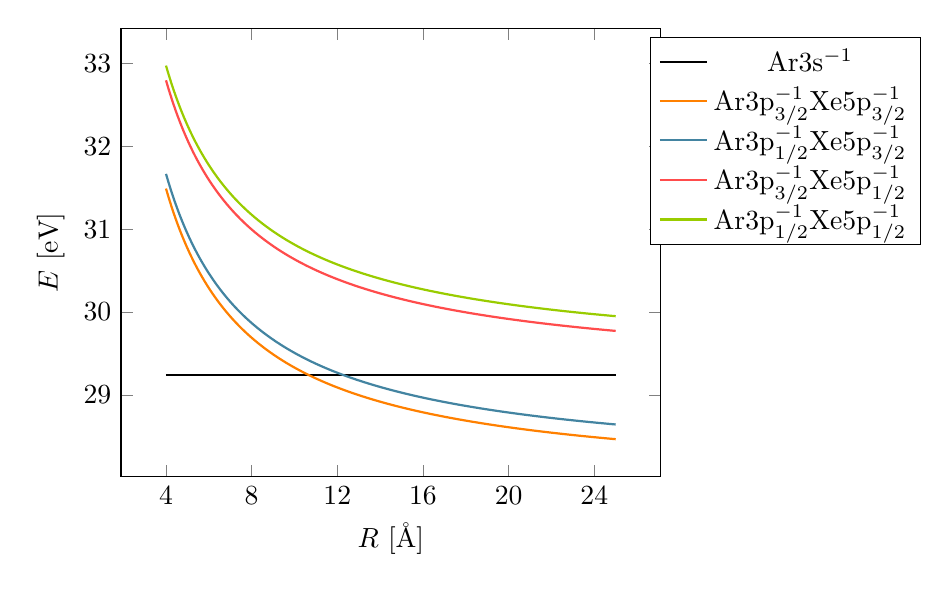
\begin{tikzpicture}
    \begin{axis}[domain=4.0:25,
                 samples = 200,
                 xtick={4.0,8.0,...,24},
                 %xticklabels={$-\pi$,$-\frac \pi 2$,0,$\frac \pi 2$,$\pi$},
                 cycle list name = exotic,
                 legend style={anchor= north west},
                 xlabel={$R$ [\AA]},
                 ylabel={$E$ [eV]}
                 ]
      \addplot+[
                mark = none,
                black,
                thick
               ]
               {29.239};
      \addlegendentry{Ar3s$^{-1}$};
      \addplot+[
                mark = none,
                thick
               ]
               {15.7596 + 12.1298 + 14.39964 / x};
      \addlegendentry{Ar3p$_{3/2}^{-1}$Xe5p$_{3/2}^{-1}$};
      \addplot+[
                mark = none,
                thick
               ]
               {15.9371 + 12.1298 + 14.39964 / x};
      \addlegendentry{Ar3p$_{1/2}^{-1}$Xe5p$_{3/2}^{-1}$};
      \addplot+[
                mark = none,
                thick
               ]
               {15.7596 + 13.4363 + 14.39964 / x};
      \addlegendentry{Ar3p$_{3/2}^{-1}$Xe5p$_{1/2}^{-1}$};
      \addplot+[
                mark = none,
                thick
               ]
               {15.9371 + 13.4363 + 14.39964 / x};
      \addlegendentry{Ar3p$_{1/2}^{-1}$Xe5p$_{1/2}^{-1}$};
      %\draw[] (axis cs:\pgfkeysvalueof{/pgfplots/xmin},29.239) -- (axis cs:\pgfkeysvalueof{/pgfplots/xmax},29.239);
    \end{axis}
\end{tikzpicture}

 \caption{}
 \label{figure:ArXe_energy_curves_unshifted}
\end{figure}

The ArXe dimer is chosen as an example for illustrating the distance
dependency of the final states compared to the initial state using
ionization energies of the corresponding atoms.
In figure \ref{figure:ArXe_energy_curves_unshifted} the energy of
the Ar3s$^{-1}$ initial
state is assumed to be constant, independent of any stabilization by the
neighbour and drawn as a black line. Additionally both the
curves of the four final states of the relativistic description and
a hypothetical non-relativistic curve calculated by the means of
equation (\ref{equation:E_fin}) are shown.

For small distances, all channels are closed. As soon as the final
state curves cross the energy of the initial state
the respective channels open. For the four relativistic channels these are
\unit[10.67]{\AA}, \unit[12.29]{\AA} and \unit[334.1]{\AA}
for the Ar3p$_{3/2}^{-1}$Xe5p$_{3/2}^{-1}$,
Ar3p$_{1/2}^{-1}$Xe5p$_{3/2}^{-1}$ and Ar3p$_{3/2}^{-1}$Xe5p$_{1/2}^{-1}$
channels, respectively.
The sum of the two ionization potentials of the
Ar3p$_{1/2}^{-1}$Xe5p$_{1/2}^{-1}$ channel are already higher than
the initial state energy. Therefore this channel never opens.
In the non-relativistic treatment, this opening distance would be
\unit[16.84]{\AA}.

Hence, for an ArXe dimer with an equilibrium distance of \unit[4.04]{\AA}
all ICD channels are closed. As is to be seen in the discussion of mixed
ArXe clusters, that in case of shifted curves, ICD channels might
open at realistic atomic distances.


\subsubsection{Geometry Dependence of the ICD Decay Widths}
